% !TEX TS-program = pdflatex
% !TEX encoding = UTF-8 Unicode

% This is a simple template for a LaTeX document using the "article" class.
% See "book", "report", "letter" for other types of document.

\documentclass[12pt]{article} % use larger type; default would be 10pt

\usepackage[utf8]{inputenc} % set input encoding (not needed with XeLaTeX)

\usepackage[numbers]{natbib}

%%% PAGE DIMENSIONS
\usepackage{geometry} % to change the page dimensions
\geometry{a4paper} % or letterpaper (US) or a5paper or....
\geometry{text={6.5in,9in}}
% \geometry{landscape} % set up the page for landscape
%   read geometry.pdf for detailed page layout information

\usepackage{graphicx} % support the \includegraphics command and options

% \usepackage[parfill]{parskip} % Activate to begin paragraphs with an empty line rather than an indent

%%% PACKAGES
\usepackage{booktabs} % for much better looking tables
\usepackage{array} % for better arrays (eg matrices) in maths
\usepackage{paralist} % very flexible & customisable lists (eg. enumerate/itemize, etc.)
\usepackage{verbatim} % adds environment for commenting out blocks of text & for better verbatim
\usepackage[margin=2cm]{caption}

%%% HEADERS & FOOTERS
\usepackage{fancyhdr} % This should be set AFTER setting up the page geometry
\pagestyle{fancy} % options: empty , plain , fancy
\renewcommand{\headrulewidth}{0pt} % customise the layout...
\lhead{}\chead{}\rhead{}
\lfoot{}\cfoot{\thepage}\rfoot{}
\newcommand{\HRule}{\rule{\linewidth}{0.5mm}}

%%% SECTION TITLE APPEARANCE
\usepackage{sectsty}
\allsectionsfont{\sffamily\mdseries\upshape} % (See the fntguide.pdf for font help)
% (This matches ConTeXt defaults)

%%% ToC (table of contents) APPEARANCE
\usepackage[nottoc,notlof,notlot]{tocbibind} % Put the bibliography in the ToC
\usepackage[titles,subfigure]{tocloft} % Alter the style of the Table of Contents
\renewcommand{\cftsecfont}{\rmfamily\mdseries\upshape}
\renewcommand{\cftsecpagefont}{\rmfamily\mdseries\upshape} % No bold!

\usepackage{array}
\newcolumntype{L}[1]{>{\raggedright\let\newline\\\arraybackslash\hspace{0pt}}m{#1}}

\usepackage{textcomp}
\usepackage{tikz}
\usetikzlibrary{calc,shapes,arrows}
\usepackage{csquotes}
\usepackage{subcaption}
\usepackage[toc,page]{appendix}
%%% END Article customizations

% -----------------------------------------------------------

\begin{document}

\begin{titlepage}
\begin{center}

\textsc{\LARGE Radboud University Nijmegen}\\[1.5cm]

% Upper part of the page. The '~' is needed because \\
% only works if a paragraph has started.

\includegraphics[width=0.15\textwidth]{images/ru-logo}~\\[1cm]

\textsc{\Large AI Master Thesis}\\[0.5cm]

% Title
\HRule \\[0.4cm]
{ \huge \bfseries Augmenting a multimodal Recurrent Neural Network  with textual context for automatically generating image descriptions \\[0.4cm] }

\HRule \\[1.5cm]

% Author and supervisor
\begin{minipage}{0.4\textwidth}
\begin{flushleft} \large
\emph{Author:}\\
Flip \textsc{van Rijn} \\
(s4050614)
\end{flushleft}
\end{minipage}
\begin{minipage}{0.4\textwidth}
\begin{flushright} \large
\emph{Supervisor:} \\
Dr.~F. \textsc{Grootjen} \\
~\\
\emph{External supervisor Dedicon:} \\
R. \textsc{Versteeg}\\
\end{flushright}
\end{minipage}

\vfill

% Bottom of the page
SOW-MKI91 AI Master Thesis\\
Artificial Intelligence\\
Faculty of Social Sciences\\
Radboud University Nijmegen\\
{\large \date{}}

\end{center}
\end{titlepage}
	
\abstract{} % TODO: Write abstract

\section{Introduction}
People with a visual impairment are not able to read text or reliably interpret visual input. For this target group special types of books, such as braille books or audio books, are made to enable these people to still perform the same task but then via a different medium. 

Similarly, user interfaces of programs on computers are often enhanced in such a way that screen readers, which are text-to-speech software, can easily read out what is being displayed on the screen. Examples of these enhancements are alternative texts for images or reorganizing the layout such that only relevant information is given to the screen reader. However, in a study about the frustrations of screen reader users on the web \citeauthor{lazar2007frustrates} \cite{lazar2007frustrates} aggregated a list of causes of frustration from 100 blind users. These users have a screen reader. This list showed that the often used enhancements, such as alternative text for images, are not always enforced by websites. The top causes of frustrations include (among others) the layout that causes out of order auditory output from the screen reader, poorly designed forms and no alternative text for images. 

The study about the frustrations of screen reader users on the web shows that one cannot rely on external sources to provide a user friendly experience, such as a well formatted layout or an additional description of the images. Not only on the web, but also in magazines or newspapers there are often images that are not or limited augmented with textual descriptions and thus are useless for people with a visual impairment. However, multiple fields within artificial intelligence, such as computer vision, machine learning and linguistics, can be used to help the end-user with providing a computer generated description of an image. 

\subsection{Related work}
Literature shows many studies involving object recognition and classification \cite{carbonetto2004statistical, he2015delving} using convolutional neural networks (CNNs). In these studies objects ranging from inanimate to animate in images are classified, which results in a label that describes to which class each object belongs to. The most recent study \cite{he2015delving} claims a performance that even surpasses human performance on classifying images. 
While this study focuses on the image classification by labeling images, other studies \cite{mao2014explain, mitchell2012midge, Yang2011, Farhadi2010} have focused on the generation of sentences from images by combining a computer vision approach with linguistic models. For description generation often two types of approaches are used in the literature. The first type is connecting the grammar of a sentence in a description to an object or a relation between objects \cite{karpathyjoulin2014deep}. Models that use this approach generate sentences for the description that are following the syntactically correctness of the language grammar. The description generation model that is mentioned in \cite{mitchell2012midge} follows this first approach. It is trained on the Flickr datasets which consists of images and descriptions. In order to generate meaningful sentences, the model uses co-occurrence statistics to compute the probability distribution within a noun phrase. Furthermore, the characteristics of visually descriptive text are inspected to determine what generally the structure is of this type of text. These statistics are then used in the model along with the computer vision input (number of objects, labels) to generate novel sentences.

The second type of approach is using probabilistic machine learning to learn the probability density over multimodal input such as text and images. These models also generate sentences for the description, but are not according to a grammar. This results into more expressive sentences, but may contain less sound grammatical structures. The models in \cite{mao2014explain,karpathyfeifei2014deep,karpathyjoulin2014deep} are according to this second approach and the authors describe the model which consists of a multimodal Recurrent Neural Network. What this network makes multimodal network is the multimodal layer. This layer connects the word representations layer with the image feature extraction network that is finally combined into a multimodal feature vector. 

\subsection{Existing model}
The overall architecture of the model that will be used is based on the model by \citeauthor{karpathyfeifei2014deep} where a CNN is combined with a Recurrent Neural Network \cite{karpathyfeifei2014deep} or by \citeauthor{vinyals2014show} where a CNN is combined with a Long-Short Term Memory (LSTM) network \cite{vinyals2014show}. Both approaches use a CNN by \citeauthor{simonyan2014very} \cite{simonyan2014very} to extract features from an image and a model which can integrate the image features and a sequence of words.  

When an LSTM model is compared to an RNN model an LSTM model tends to outperform the other model on sequence tasks such as generating sentences from images or translation \cite{vinyals2014show}. 

In the next sections the CNN is explained in more detail as well as the LSTM approach for combining the image and text.

\subsubsection{Image features}
The CNN part of the multimodal model is designed by \citeauthor{simonyan2014very}. They participated in the ImageNet Large-Scale Visual Recognition Challenge (ILSVRC) 2014 as the Visual Geometry Group (VGG) with a very deep convolution network and finished with the first and second place. Prior to their work, CNNs consisted of only a few layers and convolution filters with large receptive fields were used. However, \citeauthor{simonyan2014very} took another approach by lowering the size of the convolution filters to 3\texttimes 3 in all layers and by increasing the number of weight layers to 16 or 19. These architectures were not only able to achieve state-of-the-art accuracy on the classification and localization tasks, but were also able to generalize to other datasets.

The last layer of the model has 1000 output units that represent the 1000 categories on which the model has been trained. The activation of each of those units are probabilities for each category to be present in the image. 

In order to integrate this model in the overall multimodal model, the classification layers are stripped off to expose the rectified linear unit (ReLU) in order to get the more rich internal representation of 4096 abstract features.

\subsubsection{Combining image and text}
\citeauthor{vinyals2014show} use an LSTM model to generate sentences from images. The main component of such a model is the memory cell which contains information at every time step about the inputs that have been given up until this step. Furthermore, three binary gates govern the behavior of the model by telling the cell to forget the current value, read its input and outputting its new value. A general overview of such a model is shown in Figure~\ref{fig:lstm} where each part itself and the relation with other parts are depicted. The $\odot$ nodes indicate a multiplication with the gate values.

\begin{figure}[h!]
\centering
	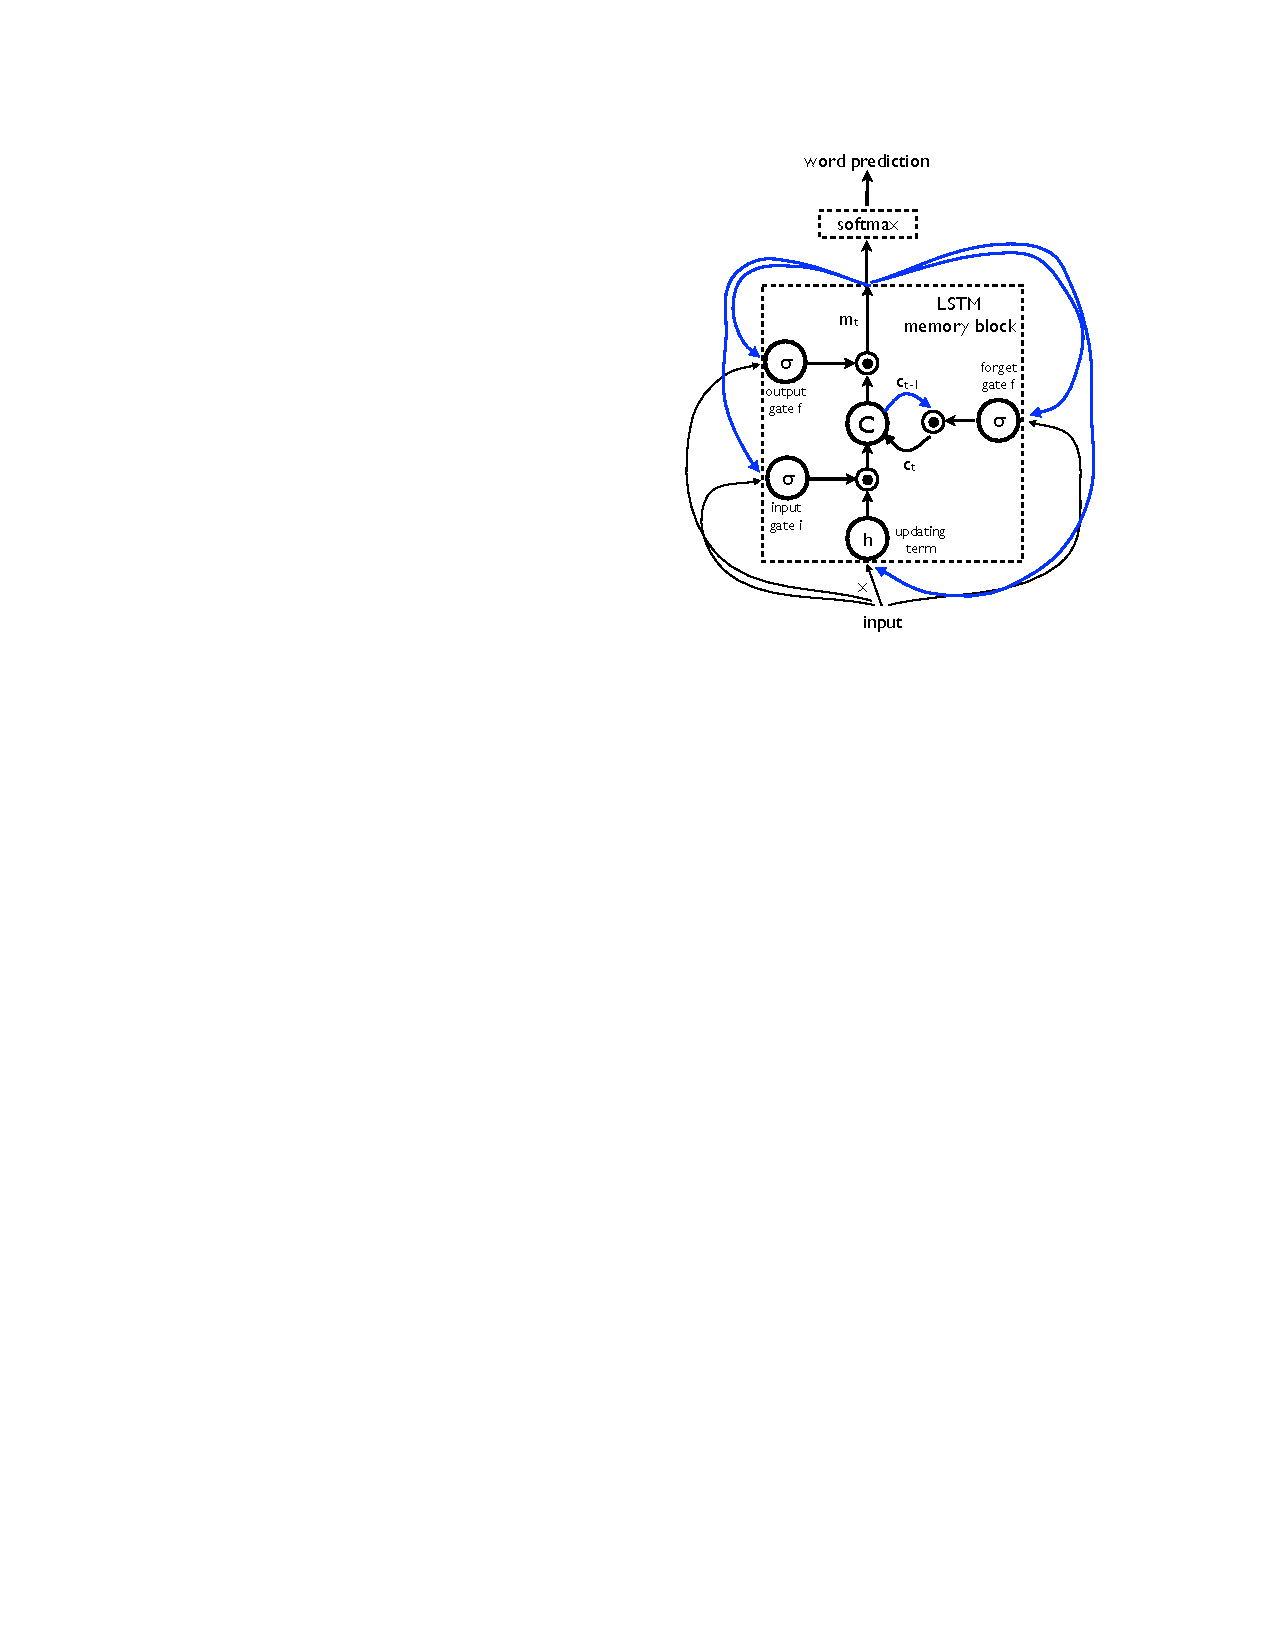
\includegraphics[width=0.5\textwidth]{images/LSTM}
	\caption{Illustration of an LSTM model adopted from \cite{vinyals2014show}: Memory cell $C$ which is controlled by three gates $\sigma_{output}$, $\sigma_{input}$ and $\sigma_{forget}$. The blue lines indicate the recurrent connections from the output $m_{t-1}$ back to the gates at time $t$.}
	\label{fig:lstm}
\end{figure}

The image $I$ is fed into the model ($x$) only at the initial step. After this step the sequence of words in the ground truth sentence $S = (S_0,\ldots,S_N)$ is the input of the model. To mark the start and the ending of the sentence, $S_0$ and $S_N$ are special tokens. The words in the sentence are encoded as a 1-of-$K$ vector, where $K$ is the number of words in the entire vocabulary (training set) and the 1 is the index of the word in the vocabulary.

\begin{equation}\label{eq:loss-function-lstm}
	L(I,S)=-\sum\limits_{t=1}^{N}\log p_t(S_t)
\end{equation}

The output of the model is a probability distribution $p_t$ over all words in the vocabulary. Finally, the loss function formalized in Equation~\ref{eq:loss-function-lstm} is minimized taking into account all the parameters of the model, the image features from the CNN and the word encodings.

\section{Methods}
\label{sec:methods}

\subsection{Dataset}
% TODO: rewrite dataset part for MSCOCO dataset
This consists of images, their descriptions and the textual context in which these images occur. Many datasets, such as ImageNET \cite{Russakovsky2012} and MSCOCO \cite{Lin2014}, exist of which many only consist of images and their description. Though, next to images and their annotations, in this approach the dataset also needs to include the context in which the image is in. In the literature the MSCOCO and/or Flickr8K/Flickr30K dataset are used for various image retrieval tasks as well as for image annotation tasks. In order to compare the models in the literature with the model in the thesis and since this dataset contains the required components to develop and train a model for automatic image description generation, either one of these datasets can be used. 

However, the textual context still is lacking in either of these datasets. Another dataset -- ImageCLEF \cite{Gilbert15_CLEF}, consisting of 500,000 images  from various sources on the internet -- does have some representation of textual context, since this dataset also contains the webpages on which the images are hosted. This can be used as the context for the images.

Since the literature mainly uses MSCOCO and/or the Flickr datasets and the results of this thesis has to be compared to earlier research, the MSCOCO dataset is used. This dataset is constructed with photos from the Flickr website. However, only the direct link to the photo is provided. Therefore, the Flickr API is used to retrieve the page the photo is on and additionally the title and the description provided by the author of the photo. 

However, the model of this thesis will be used by Dedicon and data that they have might not represent the data that is used by MSCOCO. First of all the language (English vs. Dutch) is different which will have a big impact if this model were to be trained on the MSCOCO dataset and then tested on the Dedicon dataset. Furthermore, the images in the Dedicon dataset might be of an entirely different category compared with the images in the MSCOCO dataset. Therefore, only one of the datasets can be used to both train and test the model on. Once a working prototype of the model has been created and trained, the model is tested on a subset of the dataset that is used. 

\subsection{Pre-processing}
Regularly words in a description correspond with a region in the image. This information can be used to improve the novel description generation of images. A first step in pre-processing would be to localize objects in the image which then result in bounding-boxes that describe regions of interest. Of the state-of-the-art methods that recognize objects -- such as exhaustive search \cite{zhu2010latent, felzenszwalb2010object} and selective search \cite{Sande2011} -- selective search by \citeauthor{Sande2011} repurposes segmentation for object recognition. Selective search is a much faster method that prefers approximate over exact object localization, has a high recall and permits the use of more expensive features such as bag-of-words. With this method several candidate bounding boxes are generated per image.  

The next step is using these candidates as an input for a Recurrent Convolutional Neural Network (RCNN) \cite{girshick2015fast}. In essence, the purpose of the RCNN is to score each candidate using a  localization CNN which is pre-trained on the ImageNet dataset. The network receives two inputs: a batch of images and a list of regions of interest. The output of the network is a class posterior probability distribution and bounding-box offsets relative to the candidates.

The image pre-processing pipeline is depicted in Figure~\ref{fig:image-preprocessing}.

\begin{figure}
\centering  

\tikzstyle{input} = [coordinate]
\tikzstyle{combine} = [draw, fill=blue!20, circle]
\tikzstyle{method} = [draw, fill=blue!20, rectangle, 
    minimum height=3em, minimum width=6em]
    
\begin{tikzpicture}[auto, node distance=4.5cm,>=latex']
	% image stack
	\node at 	(0.4,0.5) {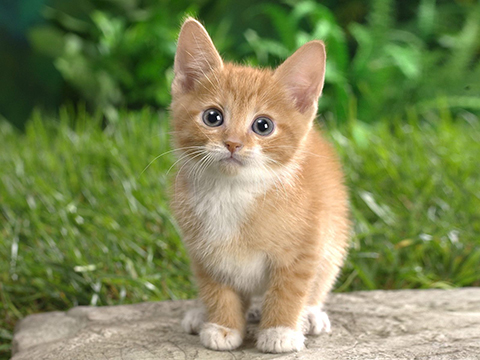
\includegraphics[width=0.04\textwidth]{images/cat}};
	\node at 	(0.25,0.65) {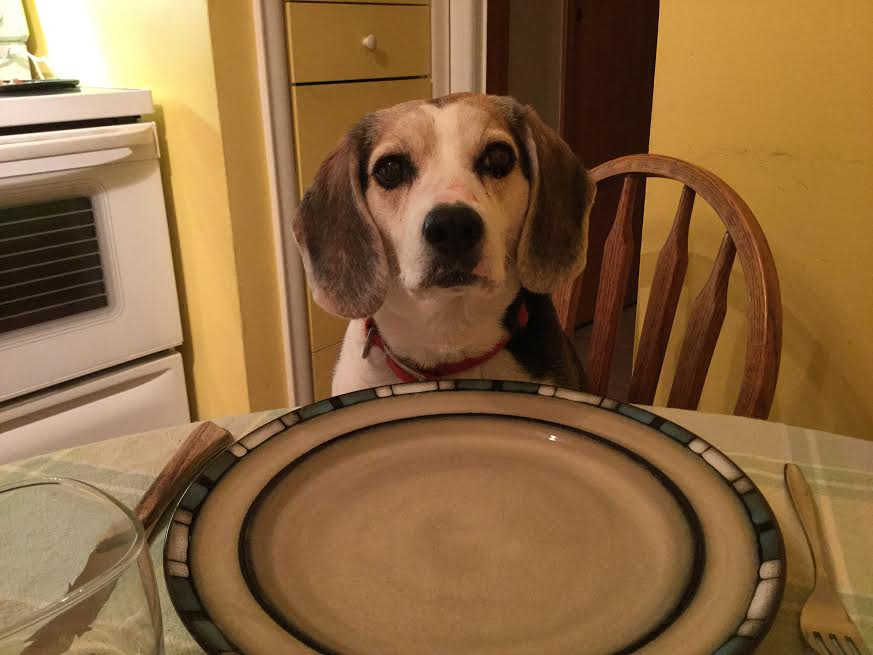
\includegraphics[width=0.04\textwidth]{images/dogdinner}};
	\node at 	(0.1,0.8) {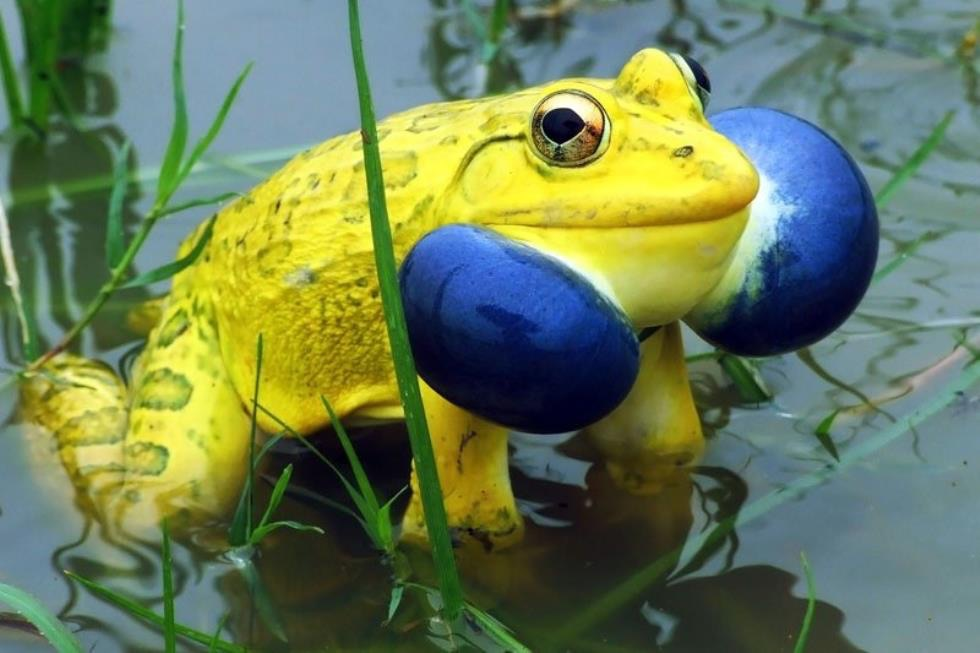
\includegraphics[width=0.04\textwidth]{images/frog}};

	\node [input, name=input] {};
	\node [combine, right of=input, node distance=1cm] (inputnode) {};
	\node [method, right of=inputnode, node distance=2.5cm]	 (selectivesearch) {selective search};
	\node [method, right of=selectivesearch, node distance=5cm] (rcnn) {RCNN};
	\node [combine, right of=rcnn, node distance=3cm] (bbox) {};
	\node [combine, right of=bbox, node distance=2cm] (roi) {};
	
	\draw [draw,->] (input) -- node {} (inputnode);
	\draw [->] (inputnode) -- node {$i$} (selectivesearch);
	\draw [->] (selectivesearch) -- node {candidates} (rcnn);
	\draw [->] (rcnn) -- node {bbox} (bbox);
	\draw (inputnode) edge[out=90, in=90, distance=2cm, below, ->] node {$i$} (bbox);
	\draw [->] (bbox) -- node {ROI} (roi);
\end{tikzpicture}
\caption{Image pre-processing pipeline. Each image $i\in I$ is processed (in batches or individually) by this pipeline resulting in regions of interest in each image.}
\label{fig:image-preprocessing}
\end{figure}

\section{Results}
\label{sec:results}

\begin{enumerate}
\item BLUE \cite{Papineni2002}
\item CIDEr-D \cite{vedantam2014cider}
\item Meteor \cite{lavie2014meteor}
\item ROUGE \cite{Lin2004a}
\end{enumerate}

\section{Discussion}
\label{sec:discussion}

\section{Conclusion}
\label{sec:conclusion}

\pagebreak

\bibliographystyle{plainnat}
\bibliography{references}

\begin{appendices}
\section{Software dependencies}
\begin{itemize}
\item Caffe, http://caffe.berkeleyvision.org/
\end{itemize}
\end{appendices}

\end{document}
